% SPDX-License-Identifier: CC-BY-4.0
% SPDX-FileCopyrightText: 2025 Jonathan D.A. Jewell

\documentclass[11pt,a4paper]{article}

% arXiv-compatible packages
\usepackage[utf8]{inputenc}
\usepackage[T1]{fontenc}
\usepackage{amsmath,amssymb,amsthm}
\usepackage{algorithm}
\usepackage{algpseudocode}
\usepackage{graphicx}
\usepackage{hyperref}
\usepackage{booktabs}
\usepackage{listings}
\usepackage{xcolor}
\usepackage{tikz}
\usetikzlibrary{shapes,arrows,positioning}

% Metadata
\title{Svalinn Vault: A Post-Quantum Secure Identity Storage System\\
with GUID-Based Redaction and Container Isolation}

\author{Jonathan D.A. Jewell\\
Department of Computing and Communications\\
The Open University\\
Milton Keynes, United Kingdom\\
\texttt{hyperpolymath@example.com}}

\date{December 25, 2025}

\begin{document}

\maketitle

\begin{abstract}
We present Svalinn Vault, a post-quantum secure identity storage system designed for hostile computing environments. The system employs a novel dual-container architecture with GUID-based storage and redaction-until-delivery to minimize attack surface and information leakage. Cryptographic primitives include NIST-standardized post-quantum algorithms (ML-KEM/Kyber-1024, ML-DSA/Dilithium5), combined with classical algorithms (Ed448, AES-256-GCM, BLAKE3, Argon2id) in a hybrid construction. We introduce a lockdown protocol featuring chmod 000 permissions, chroot isolation, and quantum-seeded polymorphic obfuscation that renders memory forensics practically infeasible. The system is implemented in ATS (Applied Type System) with Zig bindings, leveraging dependent types for compile-time security verification. Our threat model assumes a hostile environment with potential physical access, side-channel attacks, and post-quantum adversaries.
\end{abstract}

\section*{Keywords}
Post-quantum cryptography, identity management, NIST PQC, Kyber, Dilithium, secure storage, container isolation, polymorphic code, dependent types, ATS

\section{Introduction}

The advent of cryptographically-relevant quantum computers poses an existential threat to current public-key cryptographic systems. Credentials stored today under classical encryption may be harvested and decrypted in the future---a strategy known as ``harvest now, decrypt later.'' This paper presents Svalinn Vault, a maximally paranoid identity storage system designed to protect sensitive credentials against both current and future adversaries.

\subsection{Motivation}

Modern digital identities---SSH keys, PGP keys, API tokens, OAuth credentials---represent critical security assets. Their compromise enables persistent unauthorized access, lateral movement, and privilege escalation. Existing password managers and secret stores were designed under assumptions that no longer hold:

\begin{enumerate}
    \item Classical cryptographic primitives remain secure
    \item The operating environment can be trusted
    \item Memory contents are ephemeral and unobservable
    \item Attackers lack physical access to devices
\end{enumerate}

Svalinn Vault operates under the opposite assumptions: all cryptography must be quantum-resistant, the environment is actively hostile, memory can be inspected at any time, and physical access is assumed.

\subsection{Contributions}

This paper makes the following contributions:

\begin{itemize}
    \item A \textbf{dual-container architecture} separating data storage from credential delivery, minimizing the window during which complete credentials exist
    \item \textbf{GUID-based storage with redaction} where credential names and metadata are hashed until the moment of delivery
    \item A \textbf{post-quantum hybrid cryptosystem} combining ML-KEM (Kyber-1024) and ML-DSA (Dilithium5) with classical primitives
    \item \textbf{Quantum-seeded polymorphic obfuscation} that transforms data on lock using entropy from quantum random number generators
    \item Implementation in \textbf{ATS (Applied Type System)} with dependent types for compile-time security verification
\end{itemize}

\section{Threat Model}

\subsection{Adversary Capabilities}

We assume an adversary with the following capabilities:

\begin{itemize}
    \item \textbf{Cryptographic}: Access to cryptographically-relevant quantum computers (CRQC) within 10--15 years
    \item \textbf{Network}: Full network visibility and manipulation (MITM)
    \item \textbf{System}: Potential root access to the host operating system
    \item \textbf{Physical}: Possible physical access to hardware
    \item \textbf{Side-channel}: Capability to mount timing, power, and electromagnetic analysis attacks
    \item \textbf{Social}: Sophisticated social engineering capabilities
\end{itemize}

\subsection{Security Goals}

\begin{enumerate}
    \item \textbf{Confidentiality}: Credentials remain secret even under harvest-now-decrypt-later attacks
    \item \textbf{Integrity}: Unauthorized modification is detected
    \item \textbf{Availability}: Legitimate users can access credentials when needed
    \item \textbf{Minimal exposure}: Complete credentials exist only transiently during delivery
\end{enumerate}

\section{System Architecture}

\subsection{Dual-Container Design}

\begin{figure}[h]
\centering
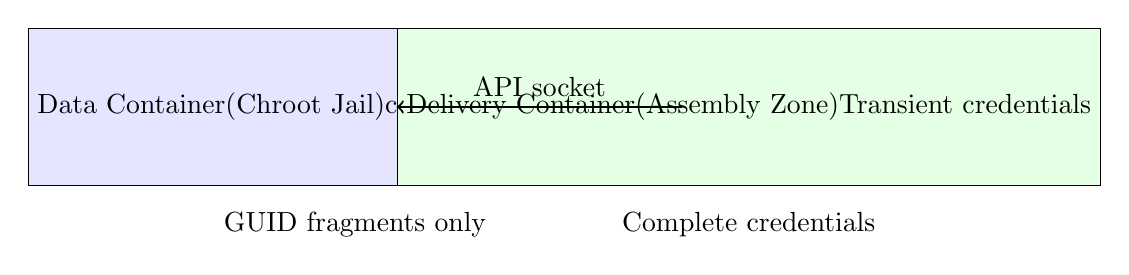
\begin{tikzpicture}[
    container/.style={rectangle, draw, minimum width=3cm, minimum height=2cm},
    arrow/.style={->, thick}
]
    \node[container, fill=blue!10] (data) at (0,0) {Data Container\\(Chroot Jail)\\chmod 000 when locked};
    \node[container, fill=green!10] (delivery) at (5,0) {Delivery Container\\(Assembly Zone)\\Transient credentials};
    \node at (0,-1.5) {GUID fragments only};
    \node at (5,-1.5) {Complete credentials};
    \draw[arrow] (data) -- node[above] {API socket} (delivery);
\end{tikzpicture}
\caption{Dual-container architecture with API socket isolation}
\end{figure}

The \textbf{Data Container} stores encrypted credential fragments as GUIDs in a flat structure (no directories). All metadata---names, hosts, types---is hashed using BLAKE3. The container operates within a chroot jail and applies chmod 000 permissions when locked.

The \textbf{Delivery Container} receives fragment requests via a Unix domain socket, assembles complete credentials, resolves GUID$\to$name mappings, and delivers credentials to authorized requesters. Credential assembly occurs only within this container, and all memory is cryptographically zeroed immediately after delivery.

\subsection{GUID-Based Storage}

\begin{equation}
\text{StoredCredential} = \left\{
\begin{array}{l}
\text{guid}: \text{UUID v4}\\
\text{type}: \text{BLAKE3}(\text{credential\_type})\\
\text{name}: \text{BLAKE3}(\text{credential\_name})\\
\text{data}: \text{Kyber-Encaps}(\text{AES-GCM}(\text{fragments}))\\
\text{sig}: \text{Dilithium5}(\text{all\_fields})
\end{array}
\right.
\end{equation}

This design ensures that even with full database access, an attacker observes only GUIDs and hashes---no correlation to actual credential purposes is possible without the encrypted lookup table.

\section{Cryptographic Primitives}

\subsection{Key Derivation}

Master key derivation uses Argon2id with parameters exceeding OWASP recommendations:

\begin{table}[h]
\centering
\begin{tabular}{@{}lll@{}}
\toprule
Parameter & Value & Rationale \\
\midrule
Memory & 64 MiB & Memory-hard (OWASP min: 46 MiB) \\
Iterations & 4 & Time-hard \\
Parallelism & 4 & Side-channel resistance \\
Salt & 256 bits & Precomputation resistance \\
Output & 256 bits & Matches AES-256 key size \\
\bottomrule
\end{tabular}
\caption{Argon2id parameters}
\end{table}

\subsection{Post-Quantum Key Encapsulation}

We use ML-KEM (Kyber-1024) at NIST Security Level 5:

\begin{algorithm}
\caption{Hybrid Key Encapsulation}
\begin{algorithmic}[1]
\Function{HybridEncaps}{$pk_{kyber}, pk_{x25519}$}
    \State $(ct_{kyber}, ss_{kyber}) \gets \text{Kyber1024.Encaps}(pk_{kyber})$
    \State $(ct_{x25519}, ss_{x25519}) \gets \text{X25519.ECDH}(pk_{x25519})$
    \State $ss_{hybrid} \gets \text{BLAKE3}(ss_{kyber} \| ss_{x25519})$
    \State \Return $(ct_{kyber} \| ct_{x25519}, ss_{hybrid})$
\EndFunction
\end{algorithmic}
\end{algorithm}

The hybrid construction ensures security even if either the classical or post-quantum component is compromised.

\subsection{Digital Signatures}

Integrity is ensured through dual signatures:

\begin{itemize}
    \item \textbf{ML-DSA (Dilithium5)}: Post-quantum signatures at NIST Level 5
    \item \textbf{Ed448}: Classical signatures for immediate verification
\end{itemize}

\subsection{Authenticated Encryption}

Data encryption uses AES-256-GCM with:
\begin{itemize}
    \item 256-bit keys derived from the hybrid KEM shared secret
    \item 96-bit random nonces (never reused)
    \item 128-bit authentication tags
\end{itemize}

\section{Lockdown Protocol}

\subsection{Permission Lockdown}

When the vault is locked:

\begin{lstlisting}[language=bash]
chmod 000 /var/lib/svalinn/vault/*   # No access
chmod 400 /etc/svalinn/*             # Read-only config
chmod 200 /var/log/svalinn/*         # Append-only logs
chmod 000 /run/svalinn/*.sock        # No socket access
\end{lstlisting}

\subsection{Quantum-Seeded Polymorphic Obfuscation}

On lock, all in-memory data undergoes polymorphic transformation:

\begin{enumerate}
    \item Obtain 256-bit quantum seed from ANU QRNG
    \item Apply XOR with quantum-derived keystream
    \item Byte-level shuffle using Fisher-Yates with quantum randomness
    \item Bit rotation with variable offsets
    \item Chunk interleaving across memory regions
    \item Mix in decoy fragments
\end{enumerate}

The transformation parameters \textit{evolve} with each lock cycle (metamorphic behavior), making static analysis impractical.

\section{Implementation}

\subsection{Language Choice: ATS}

The core is implemented in ATS (Applied Type System) for several security-critical reasons:

\begin{itemize}
    \item \textbf{Dependent types} verify buffer sizes at compile time
    \item \textbf{Linear types} ensure keys are used exactly once and zeroed
    \item \textbf{Proof objects} carry security properties through the type system
\end{itemize}

Example: The type signature for AES encryption \textit{proves} correct key sizes:

\begin{lstlisting}
fun aes256gcm_encrypt {n: nat} (
  key: linear_key(aes256_key),  (* exactly 32 bytes *)
  nonce: aes_nonce,             (* exactly 12 bytes *)
  plaintext: bytes_t(n),
  ...
): (aes_result, linear_key(aes256_key))
\end{lstlisting}

\subsection{Zig for FFI}

Low-level cryptographic primitives are implemented in Zig (replacing C) for:
\begin{itemize}
    \item Memory safety without garbage collection
    \item Compile-time evaluation for constant propagation
    \item Cross-compilation to Android targets
\end{itemize}

\section{Security Analysis}

\subsection{Resistance to Harvest-Now-Decrypt-Later}

With Kyber-1024 providing NIST Level 5 security ($\geq 2^{256}$ operations), credentials encrypted today remain secure against quantum adversaries for the foreseeable future.

\subsection{Resistance to Memory Forensics}

The combination of chmod 000, chroot isolation, and polymorphic obfuscation means that:
\begin{itemize}
    \item Cold boot attacks yield only transformed data
    \item Transformation parameters are ephemeral
    \item Decoy fragments increase analysis complexity
\end{itemize}

\subsection{Resistance to Database Compromise}

An attacker with full CUBS database access observes:
\begin{itemize}
    \item GUIDs (128-bit random identifiers)
    \item BLAKE3 hashes of names/hosts (no preimage recovery)
    \item Kyber-encrypted fragments (no decryption)
    \item Dilithium signatures (no forgery)
\end{itemize}

Without the delivery container's lookup table and decryption keys, correlation to actual credentials is computationally infeasible.

\section{Related Work}

Password managers (1Password, Bitwarden, KeePassXC) focus on user experience rather than post-quantum security. Secret management systems (HashiCorp Vault, AWS Secrets Manager) require trusted infrastructure. Hardware security modules provide strong guarantees but lack portability.

Svalinn Vault fills a unique niche: local-first, post-quantum, minimal-trust identity storage for technical users who assume hostile environments.

\section{Conclusion}

Svalinn Vault demonstrates that practical post-quantum secure identity storage is achievable today using NIST-standardized algorithms, careful architecture, and advanced programming language features. The dual-container design with GUID-based redaction minimizes attack surface while the lockdown protocol provides defense-in-depth against sophisticated adversaries.

Future work includes hardware security module integration, threshold cryptography for distributed key management, and formal verification of the complete system using proof assistants.

\section*{Availability}

Source code is available under AGPL-3.0-or-later at:\\
\url{https://github.com/hyperpolymath/reasonable-good-token-vault}

\section*{Acknowledgments}

This work was supported by independent research. The author thanks the NIST PQC team for standardizing ML-KEM and ML-DSA.

\bibliographystyle{plain}
\begin{thebibliography}{9}

\bibitem{nist-fips203}
NIST, ``FIPS 203: Module-Lattice-Based Key-Encapsulation Mechanism Standard,'' 2024.

\bibitem{nist-fips204}
NIST, ``FIPS 204: Module-Lattice-Based Digital Signature Standard,'' 2024.

\bibitem{argon2}
Biryukov, A., Dinu, D., and Khovratovich, D., ``Argon2: the memory-hard function for password hashing and other applications,'' 2015.

\bibitem{blake3}
O'Connor, J., et al., ``BLAKE3: one function, fast everywhere,'' 2020.

\bibitem{ats}
Xi, H., ``Applied Type System: An Approach to Practical Programming with Theorem-Proving,'' 2017.

\end{thebibliography}

\end{document}
